\part{Recherche binaire}
  L'objectif de cette partie est de mesurer la complexité algorithmique d'une recherche par dichotomie.

  \section{Paramètres expérimentaux}

    Les paramètres ont été changé par rapport à toutes les autres mesures : nous avons pris des tableau de valeurs
     de tailles alant de 0 à 10000, échelonnées par palier de 100 valeurs. Afin d'apporter de la répétabilité à nos mesures,
     nous avons constamment recherché l'index du chiffre zéro dans les tableaux générés.

  \section{Résultat expérimental}

    Le résultat obtenu après avoir lancé notre programme est le graphique suivant :

    \begin{center}
      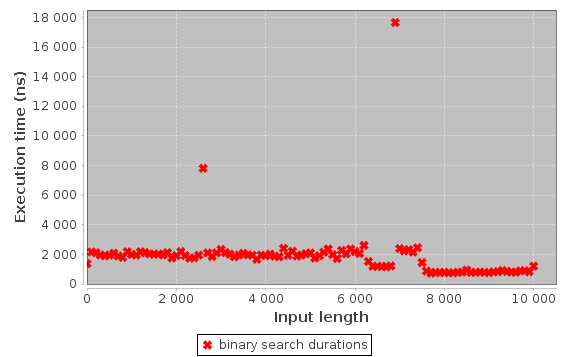
\includegraphics[width=13cm]{binarySearch}
    \end{center}

    Ce graphique est difficilement exploitable. Par ailleurs, plusieurs tentatives ont été menées pour faire varier les paramètres
    expérimentaux, et se sont toutes révéles infructueuses.
